\documentclass[12pt,a4paper]{report}

\usepackage{etoolbox}% http://ctan.org/pkg/etoolbox

\usepackage{lmodern} % add the missing package for font shapes
\usepackage[]{qcircuit}

\setcounter{secnumdepth}{1}
\renewcommand\familydefault{\sfdefault} % sans serif

\usepackage[margin=2.54cm]{geometry}	% dimensiuni pagină și margini
\usepackage{graphicx} % support the \includegraphics command and options

% formatting sections and subsections
\usepackage{textcase}
\usepackage[titletoc, title]{appendix}
\usepackage{titlesec}
\titleformat{\chapter}{\large\bfseries\MakeUppercase}{\thechapter}{3ex}{}[\vspace*{-1.5cm}]
\titleformat*{\section}{\large\bfseries}
\titleformat*{\subsection}{\large\bfseries}
\titleformat*{\subsubsection}{\large\bfseries}

\usepackage{chngcntr}
\counterwithout{figure}{chapter} % no chapter number in figure labels
\counterwithout{table}{chapter} % no chapter number in table labels
\counterwithout{equation}{chapter} % no chapter number in equation labels

\usepackage{booktabs} % for much better looking tables
\usepackage{url} % Useful for inserting web links nicely
\usepackage[bookmarks,unicode,hidelinks]{hyperref}

\usepackage{array} % for better arrays (eg matrices) in maths
\usepackage{paralist} % very flexible & customisable lists (eg. enumerate/itemize, etc.)
\usepackage{verbatim} % adds environment for commenting out blocks of text & for better verbatim
\usepackage{subfig} % make it possible to include more than one captioned figure/table in a single float
\usepackage{enumitem}
\setlist{noitemsep}

%%% HEADERS & FOOTERS
\usepackage{fancyhdr}
\pagestyle{empty}
\renewcommand{\headrulewidth}{0pt}
\renewcommand{\footrulewidth}{0pt}
\lhead{}\chead{}\rhead{}
\lfoot{}\cfoot{\thepage}\rfoot{}



\newcommand{\HeaderLineSpace}{-0.25cm}
\newcommand{\UniTextEN}{POLYTECHNIC UNIVERSITY OF BUCHAREST \\[\HeaderLineSpace]
FACULTY OF AUTOMATIC CONTROL AND COMPUTERS \\[\HeaderLineSpace]
COMPUTER SCIENCE AND ENGINEERING DEPARTMENT\\}
\newcommand{\DiplomaEN}{BACHELOR THESIS}
\newcommand{\AdvisorEN}{Thesis advisor:}
\newcommand{\BucEN}{BUCHAREST}

\newcommand{\frontPage}[6]{
\begin{titlepage}
\begin{center}
{\Large #1}  % header (university, faculty, department)
\vspace{50pt}
\begin{tabular}{p{4.15cm}p{6cm}p{4.15cm}}
\vspace{-1pt}

\includegraphics[scale=0.12]{pics/upb.png} &
\vspace{-6.5pt}
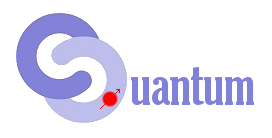
\includegraphics[scale=0.6]{pics/LogoIQC.png} &
\vspace{-2pt}

\includegraphics[scale=0.22]{pics/cs.png}
\end{tabular}

\vspace{68.5pt}
{\Huge #2}\\                           % diploma project text
\vspace{40pt}
{\Large #3}\\ \vspace{25pt}  % project title
{\Large #4}\\                          % project subtitle
\vspace{40pt}
{\LARGE \Name}\\                   % student name
\end{center}
\vspace{60pt}
\begin{tabular*}{\textwidth}{@{\extracolsep{\fill}}p{6cm}r}
&{\large\textbf{#5}}\vspace{10pt}\\      % scientific advisor
&{\large \Advisor}                                    % advisor name
\end{tabular*}
\vspace{20pt}
\begin{center}
{\large\textbf{#6}}\\                                % bucharest
\vspace{0pt}
{\normalsize \Year}
\end{center}
\end{titlepage}
}

\newcommand{\frontPageEN}{\frontPage{\UniTextEN}{\DiplomaEN}{\ProjectTitleEN}{\ProjectSubtitleEN}{\AdvisorEN}{\BucEN}}

\linespread{1.1}
\setlength\parindent{0pt}
\setlength\parskip{.23cm}

%% Abstract macro
\newcommand{\AbstractPage}{
\begin{titlepage}
\vspace*{-55pt}
{\large \textbf{ABSTRACT}}\vspace{15pt}\\
\AbstractEN \vfill
\end{titlepage}
}

%% Thank you macro
\newcommand{\ThanksPage}{
\begin{titlepage}
\vspace*{-55pt}
{\large \textbf{ACKNOWLEDGEMENTS}}\vspace{15pt}\\
\Thanks \vfill
\end{titlepage}
}



%%%%%%%%%%%%%%%%%%%%%%%%%%%%%%%%%%%%%%%%%%%%%%%%%%   
%%
%%          End of template definitions
%%   
%%%%%%%%%%%%%%%%%%%%%%%%%%%%%%%%%%%%%%%%%%%%%%%%%%


%%% Puteți elimina aceste linii din lucrare, servesc numai pentru template.
\newcommand{\worktype}[1]{[\textit{#1}] }
\newcommand{\dezvoltare}{\worktype{Dezvoltare de produs}}
\newcommand{\cercetare}{\worktype{Cercetare}}
\newcommand{\ambele}{\worktype{Ambele}}
%%%


%%
%%   Campurile de mai jos trebuie modificate de autor. Modificati doar continutul, nu si numele fiecarei definitii
%%
\newcommand{\ProjectTitleEN}{A comprehensive study on Integrating Quantum Physics in Deep Learning Models for Optimizations in Computer Vision and Natural Language Processing Fields}
\newcommand{\ProjectSubtitleEN}{QRKT-GAN: Neural Ordinary Differential Equation-Inspired Generative Adversarial Network Model with Numerical Runge-Kutta Methods for Quantum Visual Transformer-Based Generator and Discriminator}
\newcommand{\Name}{Cătălin-Alexandru Rîpanu}
\newcommand{\Advisor}{Șl. dr. ing. Dumitru-Clementin Cercel}
\newcommand{\Year}{2024}

% Setări document
\title{Diploma Project}
\author{\Name}
\date{\Year}

%%
%%   Campurile aferente rezumatului
%%

\newcommand{\AbstractEN}{Deep Learning models, such as Generative Adversarial Networks (GANs)~\cite{goodfellow2014generative} and Visual Transformers (ViTs)~\cite{vaswani2017attention}, have demonstrated remarkable results across various domains in Machine Learning and Artificial Intelligence, including Object Classification, Image Segmentation, Sentiment Analysis, and Machine Translation. These models are pivotal in advancing systems that require high precision and a deep understanding of complex data across a variety of tasks in both Natural Language Processing (NLP) and Computer Vision (CV).

However, the effectiveness of Deep Learning models comes with significant challenges: they require an extensive number of parameters to learn and extract meaningful features from real-world data. Additionally, these models need vast amounts of information to achieve desired performance levels. Obtaining such large sets can be difficult as real-world data is often not publicly available and can be challenging to collect and curate. This results in substantial computational resource requirements for both training and hyperparameter optimization, often achieved through exhaustive techniques such as grid search.

To address these challenges, this thesis proposes a novel hybrid Generative Adversarial Network architecture that employs Quantum Visual Transformers (QViTs) as both the Generator and Discriminator. Visual Transformers are selected for their superior ability to manage intricate data representations. A key innovation in this architecture is the integration of Ordinary Differential Equation (ODE)~\cite{fan2024Quantum} solvers as Encoders, enhancing the model's capability to capture temporal dynamics and complex data structures, and improving the residual connections within the transformer architecture to mitigate the vanishing gradients problem even more.

Moreover, this architecture incorporates Variational Quantum Circuits~\cite{cerezo2021variational} within both the Self-Attention Mechanisms~\cite{voita2019analyzing} and the Multi-Layer Perceptrons (MLPs)~\cite{popescu2009multilayer} of the Visual Transformers. By leveraging the principles of Quantum Mechanics, these Quantum circuits can perform complex algebraic operations more efficiently than classical methods, offering a significant computational advantage.

The performance of this hybrid model is benchmarked against SoTA purely classical baselines and configurations from the literature using datasets from both CV and NLP areas. Specifically, the model is tested on CIFAR-10~\cite{Krizhevsky09learningmultiple}, CIFAR-100~\cite{Krizhevsky09learningmultiple}, MNIST~\cite{lecun2010mnist}, IMDb Reviews~\cite{maas-EtAl:2011:ACL-HLT2011} and ILSVRC 2012~\cite{ILSVRC15}  datasets. The Quantum model is successfully trained and tested through numerical simulations. The results indicate that this hybrid approach achieves comparable classification and generation performance to the classical baseline, while requiring fewer trainable parameters.

Furthermore, the reduced parameter count in this hybrid model opens up the possibility of running it on real Quantum hardware for both training and inference. This feasibility is a significant breakthrough, as it implies that Quantum-enhanced models can be trained and deployed on actual Quantum computers, which are currently limited in terms of the number of qubits and operational fidelity.

This thesis demonstrates the potential of integrating Quantum Computing, especially Quantum mechanics, with advanced Deep Learning architectures to create more efficient and powerful networks which can significantly reduce computational costs while maintaining high performance, paving the way for more scalable and effective AI applications.}

%%
%%   Campurile aferente paginii de multumiri
%%
\newcommand{\Thanks}{
First and foremost, I would like to express my deepest gratitude to my advisor, Prof. Dumitru-Clementin Cercel, for his unwavering support and insightful guidance throughout my research journey. His expertise and encouragement have been essential in exploring the intricate intersection of Artificial Intelligence and Quantum Mechanics, widely referred to in the literature as Quantum Artificial Intelligence. This interdisciplinary field, though initially daunting, is at the cutting edge of technological advancement and innovation in both areas.

I am also profoundly thankful to Prof. Pantelimon-George Popescu for his advice, recommendations, and exceptional lectures on Quantum Computing. His mentorship has been instrumental in building a robust understanding of this groundbreaking paradigm, which promises new solutions to problems previously deemed insurmountable by classical methods.

Furthermore, I wish to acknowledge the significant contributions of the academic teaching assistants and collaborators encountered during my bachelor's studies. Their guidance during challenging times has been crucial to my academic development. Last but not least, I am also grateful for the computational resources provided by the Computer Science and Engineering Department, which were essential for the design and implementation of this project.

In addition, I extend my appreciation to my friends for their continuous support, ideas, and advice, especially during moments when inspiration was scarce. Lastly, my heartfelt thanks go to my parents for their enduring sacrifices and unwavering support throughout this journey into the unknown. Their belief in me has been a constant source of motivation.
}

\makeatletter
\def\@makechapterhead#1{%
  \vspace*{-55\p@}%
  {\parindent \z@ \raggedright \normalfont
  \ifnum \c@secnumdepth >\m@ne
  \Large\bfseries \thechapter\space% Adjust the size as needed
  \fi
  \interlinepenalty\@M
  \Large \bfseries #1\par\nobreak
  \vskip 12\p@
  }}
  
\makeatother

\begin{document}

\setcounter{page}{1}
\frontPageEN


\setcounter{page}{2}
\ThanksPage \pagestyle{fancy}

\AbstractPage\pagestyle{fancy}

\renewcommand{\contentsname}{\vspace{-3.45cm} CONTENTS}
\tableofcontents
% Textul licentei incepe de aici 

\chapter{Introduction}\pagestyle{fancy}

\section{Context}\vspace{-12pt}
Artificial Intelligence models, particularly Deep Learning ones, have made significant contributions to solving real-world tasks, greatly improving human lives in various fields, such as Medical Image Recognition~\cite{he2020infusing}. Despite their impressive capabilities, Deep Learning models come with substantial drawbacks regarding computational resources and effort. Achieving high performance with these models necessitates learning millions to billions of parameters, also called weights or artificial neurons, which demands considerable resources and preparation time. This limitation also has negative environmental impacts due to high power consumption.

Over the years, researchers have developed numerous solutions to mitigate the problem of minimizing the number of parameters using interesting classical algorithms and techniques. These include, for example, specialized activation functions for neural layers like Rectified Linear Unit~\cite{NIPS2017_a96b65a7}, Leaky ReLU~\cite{xu2020reluplex}, Gaussian Error Linear Unit~\cite{hendrycks2016gaussian}, Softmax~\cite{liu2016large}, Sigmoid~\cite{han1995influence} and Hyperbolic Tangent~\cite{zamanlooy2013efficient}. Additionally, effective optimizers such as Adam~\cite{zhang2018improved} and Stochastic Gradient Descent~\cite{bottou2010large} have been utilized to combat this limitation, along with methods like Learning Rate Schedulers~\cite{wen2021convolutional}, Weight Decay~\cite{loshchilov2017decoupled}, and Dropout~\cite{srivastava2014dropout} to reduce also the chances of model overfitting. Over the years, various architectural designs and network combinations have emerged to address these challenges. However, the tradeoff between high computational resource consumption and performance remains a difficult issue, especially when scaling up the dimensions of available noisy real-world datasets used for training. It is unlikely\footnote{\url{https://www.theverge.com/24066646/ai-electricity-energy-watts-generative-consumption}} to be efficiently resolved in the near future using solely classical approaches.

A segment of Computer Science researchers, in collaboration with physicists, have taken a bold and innovative approach to these challenges by exploring solutions from a physical perspective, leading to the emergence of Quantum Computation and Quantum Information~\cite{nielsen2001quantum}. Leveraging the principles of Quantum mechanics, AI research has begun to explore Deep Learning optimizations using Quantum elements, such as Variational Quantum Circuits~\cite{cerezo2021variational}, to develop hybrid Deep Learning models. By combining classical and Quantum methodologies, new experiments can be conducted to address performance and resource demands more efficiently, thus utilizing the unique capabilities of Quantum hardware. This involves training these models on it, also known as Parameterized Quantum Circuits~\cite{benedetti2019parameterized}, where the parameters are referred to as the qurons of the Quantum model.

Quantum Computing leverages properties like superposition and entanglement, enabling the execution of complex algebraic operations that are infeasible for classical computers. Quantum algorithms, such as Grover's Algorithm~\cite{shi2017coherence}, Quantum Phase Estimation~\cite{o2019quantum}, Quantum Fourier Transform~\cite{weinstein2001implementation} and Deutsch-Jozsa Quantum Parallelism~\cite{gulde2003implementation} provide exponential speedups for certain tasks. Integrating these Quantum principles with Deep Learning can significantly reduce the number of parameters and computational resources required while maintaining or even enhancing model performance. This interdisciplinary approach, also known as Quantum Artificial Intelligence, opens up exciting possibilities for the future of AI, promising advancements that could transform how complex problems are approached and solved in ways that classical computers, with their current architecture, could never achieve.
\section{Problem}\vspace{-12pt}
Over the years, numerous algorithms, techniques, network architectures, and methodologies have been proposed in the field of Deep Learning to tackle a wide array of tasks, such as Object Classification, Synthetic Data Generation and Detection, across various domains including Natural Language Processing, Computer Vision, Domain Adaptation, and Knowledge Distillation. These approaches have achieved high performance metrics like Accuracy, Area Under the Curve (AUC), Receiver Operating Characteristic (ROC), and F1 scores. The advent of High Performance Computing (HPC) facilities, particularly classical parallelism, has enabled Deep Learning models to process billions of examples from noisy real-world datasets effectively, thus yielding impressive results.

Despite these advancements, a significant drawback persists: the enormous number of neurons and the corresponding computational resources required by these models. Traditional solutions in classical Deep Learning, such as Cross Validation~\cite{berrar2019cross}, Hyperparameter Tuning techniques like Grid Search~\cite{liashchynskyi2019grid}, Random Search~\cite{liashchynskyi2019grid}, or Keras Tuner~\cite{pon2021hyperparameter}, and Layer Augmentation until model performance plateaus or overfits, are commonly employed. To mitigate overfitting, regularization techniques such as Ridge~\cite{ogutu2012genomic}, Lasso~\cite{ogutu2012genomic}, Elastic-Net~\cite{ogutu2012genomic} or Dropout~\cite{srivastava2014dropout} can be applied. However, these methods often involve exhaustive hyperparameter searches, which are extremely time-consuming, especially when dealing with validation sets comprising billions of data points for complex tasks. Additionally, one can apply group sparsity regularizers on network parameters, where each group acts on a single neuron, thus reducing the number of parameters by up to 80\%~\cite{alvarez2018learning} while retaining or even improving the network accuracy.

Another method employed to address these challenges is Transfer Learning~\cite{weiss2016survey}, which involves finding and loading a pretrained model as a starting point and then fine-tuning it on a specific dataset. This approach can help achieve good performance with less effort on architecture design and expedite the training process. However, the availability of suitable pretrained models is limited, and fine-tuning may yield only decent, if not disappointing, results, due to differences in the data distributions between the pretraining and fine-tuning datasets.

The primary challenge lies in balancing time and power consumption on classical systems to make robust and valid neural architectural choices. Furthermore, reducing the number of neurons too drastically is not a solution as it can lead to underfitting and degraded performance, making it difficult to solve complex and challenging tasks efficiently. The iterative process of tuning hyperparameters and optimizing model architectures is computationally intensive and often results in a significant trade-off between resource consumption and model performance.

Moreover, the reliance on vast amounts of training data for achieving desired performance further exacerbates these issues. Real-world datasets are often difficult to obtain and may not be publicly available, which complicates the development and fine-tuning of effective Deep Learning models. The extensive time and computational costs associated with hyperparameter optimization and model training present significant obstacles to advancing AI capabilities while maintaining efficiency and sustainability. This trade-off between computational resource consumption and performance remains a persistent and challenging problem in the field of Deep Learning, highlighting the need for innovative solutions that can overcome these limitations.

\section{Objective}\vspace{-12pt}
In the current landscape of Deep Learning research, there is an ongoing investigation into whether integrating models into a purely Quantum environment can significantly reduce power consumption and the number of trainable parameters without sacrificing performance. This exploration leverages techniques such as the Ansatz~\cite{hadfield2019Quantum} and Variational Quantum Circuits~\cite{cerezo2021variational}. As classical supercomputers continue to increase in power to accommodate newer, more complex deep models, their power consumption scales almost exponentially. Conversely, while the computational power of Quantum machines scales exponentially, their power consumption scales linearly. This interesting information presents a compelling case for Quantum Computing: once Quantum computers achieve fault tolerance, qubits could be efficiently used as artificial neurons in neural networks. Quantum-inspired techniques could allow networks to operate with a vast number of neurons per layer at minimal energy cost, thereby significantly reducing overall energy consumption\footnote{\url{https://www.eetimes.eu/how-Quantum-Computing-can-help-make-ai-greener/}}.

Building on the challenges outlined in the above section, the primary goal of this thesis is to explore Deep Learning models, both pure Quantum and hybrid, that leverage neural ODE-based architectures~\cite{zhong2022neural} inspired by non-trivial Variational Quantum Circuits~\cite{cerezo2021variational} within the context of Visual Transformers~\cite{vaswani2017attention} and their complex Encoders~\cite{hinton2011transforming} and Decoders~\cite{breuckmann2018scalable}. The most important objective is to minimize the number of parameters used by deep network layers utilizing the idea of replacing classical linear projection layers in Multi-Head Attention~\cite{voita2019analyzing} subroutines and Multi-Layer Perceptrons~\cite{popescu2009multilayer} with Quantum Circuits. Additionally, low truncation error Neural Ordinary Differential Equation~\cite{zhong2022neural}\cite{li2022ode} techniques will be employed to further optimize Transformer Layers, namely Runge-Kutta Methods~\cite{butcher1996history} of 1st, 2nd, 3rd, and 4th order. An analysis of Runge-Kutta 4th order method optimization which is not theoretically grounded in standard RK methods, but in terms of learning, will also be included~\cite{li2022ode}.

To better understand the rationale and motivation behind the proposed Deep Learning model in this paper, it is necessary to compare these Quantum ODE-based Transformers configurations  with their classical counterparts using datasets mentioned in the Abstract. The model utilizing the optimized Runge-Kutta 4th order method will be leveraged within the context of Vision Transformers (ViTs)~\cite{vaswani2017attention} and integrated into a Generative Adversarial Network (GAN)~\cite{goodfellow2014generative} architecture. In this configuration, both the Generator and Discriminator will be Quantum Visual Transformers\footnote{\url{https://openreview.net/pdf?id=p7xPXoKB0H}}, incorporating the optimized Neural ODE solver to generate realistic and informative synthetic data without being limited to specific types of distributions. This will be achieved using techniques such as Data Augmentation~\cite{zhao2020diffaugment} and Image Recognition at Scale~\cite{dosovitskiy2020} in the context of ViTs~\cite{vaswani2017attention}.

The final proposed architecture in this thesis, named QRKT-GAN, will be tested on a real-world consistent dataset, namely CIFAR-10~\cite{Krizhevsky09learningmultiple}, and compared using the same data with a renowned classical counterpart, TransGAN~\cite{jiang2021transgan}, which is a strong architecture built entirely free of Convolutions. This comparative analysis will provide another argument for the possible advantages of integrating Quantum Computing with advanced Deep Learning neural networks under the right context.
\section{Paper Structure}\vspace{-12pt}
The next chapter delves into the most relevant and important classical and Quantum algorithms and techniques developed over the years to leverage both Quantum and hybrid logic in Deep Learning for model optimization. This chapter will illustrate how these both hybrid and pure Quantum neural networks are designed to be compatible with real Quantum hardware provided by specialized vendors such as IBM~\cite{Santos_2016}, Google~\cite{kalai2023googles}, Microsoft~\cite{Mykhailova_2023}, and Amazon~\cite{Reyes_2021}. It will explore the advancements that make it possible to run complex Deep Learning models on Quantum computers, highlighting the interplay between Quantum Computing and Deep Learning for neural depth decreasing while not losing too much performance.

Section three will discuss the foundational concepts of Artificial Intelligence, Machine Learning, and Deep Learning. It will also provide a comprehensive overview of Quantum Computation and Quantum Information~\cite{nielsen2001quantum}, and will also introduce the emerging field of Quantum Artificial Intelligence~\cite{dunjko2018machine}. This section aims to explain how Quantum principles can enhance the capabilities of AI solutions in addressing high-demanding tasks, some of which are classified as NP-Hard~\cite{chatterjee2024solving} or NP-Complete~\cite{furer2008solving}. By understanding these fundamentals, the reader will gain insight into the potential synergies between Classical and Quantum Computing, which together form a duality in the world of Artificial Intelligence.

Section four will present an in-depth analysis of the proposed Ordinary Differential Equation-based Quantum neural networks. This includes their motivation, underlying concepts, Mathematical and Quantum frameworks, physical limitations, and future potential within their problem domain environment. The chapter will also discuss the new ODE-based GAN architecture in detail, explaining how it incorporates the traversed knowledge to minimize the solution of the optimization problem outlined in the Context subsection, while maintaining acceptable performance in Synthetic Data Generation.

The fifth chapter will detail the methodologies adopted for conducting the experiments. This includes a comprehensive description of the datasets used, their internal characteristics, and the reasons for their selection. It will compare various Quantum ODE-based configurations with their classical counterparts to fully understand the benefits and limitations of Quantum-enhanced models. Additionally, the chapter will provide a detailed comparison between the proposed QRKT-GAN model and its classical baseline, TransGAN~\cite{jiang2021transgan}, using the CIFAR-10~\cite{Krizhevsky09learningmultiple} dataset. This analysis will highlight the benefits and challenges of integrating Quantum Computing into Deep Learning, presenting it as a viable solution for specific optimization problems.

The final chapter will summarize the main ideas presented in the thesis, highlighting the relevance of the results and drawing key conclusions. It will also propose future work and outline potential directions for further research in the field of Quantum Deep Learning models, focusing on power consumption and performance optimization. This chapter will emphasize the importance of continued exploration in combining Quantum Computing with Machine Learning to achieve more robust, efficient and powerful Artificial Intelligence solutions.

\chapter{Related Work}\vspace{-12pt}
The relentless demand for improving human lives continues unabated, with increasingly complex and data-intensive needs emerging. This necessitates the development of sophisticated models capable of delivering accurate and reliable results. However, the complexity and depth of these models often result in significantly high computational resource consumption, which has environmental implications due to the energy required for such intensive processing.

Over the years, numerous classical, Quantum, and hybrid methods have been proposed to address the optimization problem of minimizing model depth without significantly sacrificing performance. One notable approach is real-time learning of the number of neurons in deep networks using structured sparsity during training, which dynamically adjusts the network structure to optimize performance without excessive resource use~\cite{alvarez2018learning}. Another method involves crafting specialized architectures that maintain a constant computational budget while slightly increasing depth to improve performance. This is achieved by dimensionality reduction before applying expensive Convolutions~\cite{wen2021convolutional} with larger patch sizes~\cite{Szegedy_2015_CVPR}. Unfortunately, Convolutions~\cite{wen2021convolutional} have been demonstrated~\cite{cordonnier2020relationship} to be less effective in capturing global feature interactions, focusing primarily on local patterns in Image Processing, compared to the Self-Attention~\cite{voita2019analyzing} mechanism utilized in Transformers~\cite{vaswani2017attention}.

In addition, some techniques focus on minimizing weights during training by splitting network weights into sets or hierarchies of multiple groups, each using disjoint sets of features. This allows parallelization, even in an embarrassingly manner, as each subnetwork operates independently, enhancing computational efficiency~\cite{pmlr-v70-kim17b}. Alternatively, population-based heuristic algorithms, such as Particle Swarm Optimization (PSO), have shown promise in optimally determining the number of parameters without exhaustive searches like grid search~\cite{liashchynskyi2019grid}, and thus saves valuable computational resources during the tuning process of these Deep Learning models~\cite{7986470}. Another approach involves reducing model parameters in deep neural networks via product-of-sums matrix decompositions, which decompose linear operators as a product of sums of simpler linear operators~\cite{wu2018prodsumnet}. For Deep CNN models, kernel-sharing between multiple convolutional layers can also be applied. Kernel-sharing is possible only between “isomorphic” layers, i.e., layers having the same kernel size, input, and output channels~\cite{azadbakht2022drastically}.

Despite their advantages, these classical methods have inherent drawbacks. Designing neural architectures from scratch to meet specific requirements is challenging and time-consuming. Moreover, methods like Particle Swarm Optimization~\cite{7986470} require optimization of additional parameters, such as activation functions~\cite{han1995influence}~\cite{NIPS2017_a96b65a7}~\cite{xu2020reluplex} and the number of epochs, to be truly effective. Quantum Neural Networks (QNNs)~\cite{abbas2021power} and Quantum Algorithms~\cite{cerezo2021variational} offer new avenues for addressing these limitations, providing potential solutions for power-efficient Deep Learning. Various Quantum frameworks, technologies, GPU-based numerical simulators, and access to real hardware have been developed to facilitate the implementation of Quantum phenomena in Machine Learning.

However, the Quantum approach shares a common challenge with classical methods: the need for specific adaptations for each type of Deep Learning model.
In the classical domain, the entire architectural framework must be meticulously analyzed to prevent performance degradation. In Quantum domain, constructing valid Variational Quantum Circuits (VQCs)~\cite{benedetti2019parameterized} that efficiently mimic classical model functions is crucial to avoid the same pitfalls.
\chapter{Background}\pagestyle{fancy}

\chapter{Proposed Solution}\pagestyle{fancy}

\chapter{Experiments}\pagestyle{fancy}

\chapter{Conclusions and Future Work}\pagestyle{fancy}

\chapter{Bibliography}\pagestyle{fancy}

\bibliographystyle{unsrt}

\begingroup
\def\chapter*#1{}
\bibliography{bibliography}
\endgroup

\end{document}
